%THEORY
\chapter[XQuery -- The XML Query Language]{XQuery \\ \huge-- The XML Query Language}
\label{chapter:theory}
XML is a markup language that can be used for encapsulating structured and
semistructured documents, relational data, and object repositories. A query
language capable of querying XML data may thus be capable of querying across
all these kinds of data sources. In this chapter we will outline the basics of
such a language, the XQuery XML query language, as well as the current state of
research and implementations. 

\section{XQuery}

XQuery is a query language developed by the XML Query working group of W3C.
Version 1.0\cite{w3c00} became a W3C Recommendation January 2007. It was designed as a
response to an emerging task: to intelligently express queries in theincreasing
amounts of information stored, exchanged and presented using XML. The language
is derived from Quilt\cite{quilt_queryLanguage}.


\begin{itemize}
\item itroduksjon
\item historie
\item bruksomr\aa der
\item ...
\item atomic vs sequence
\end{itemize}

\subsection{Basics}
\begin{itemize}
  \item sekvenser og ting atomisk, alt je
  \item andre ting som er basisk og ikke surt
\end{itemize}

\subsection{Path Expressions}
\begin{itemize}
\item fra XPath / brukt i mange andre ting (XSLT yeye)
\item ...
\item akser
\item predikat
\item semantikk 
\item eksikveringsorden etc
\end{itemize}

\subsection{FLWOR}

\begin{itemize}
\item motiv
\item ...
\item F L W O R semantikk
\item \^{} --- eksikveringsorden etc
\end{itemize}

\subsection{Binary Operators}

\begin{itemize}
\item motiv
\item ...
\item semantikk
\item hva er sant, hva er usant?
\end{itemize}



\subsection{Evt andre ting fra XQuery vi kommer til \aa~implementere}

\begin{itemize}
\item if then else

\end{itemize}

\subsection{Full Text Extensions}

\begin{itemize}
\item motiv
\item ...
\item semantikk
\item hva har man? ftcontains er kilden...
\end{itemize}
% State of the art, nåværende teknologi og implementasjoner
\section{Current state of XQuery}
\underline{\textbf{\LARGE //TODO:}} Kapittelet m\aa~fylles ut og omstruktureres

There exist a number of XQuery implementations, few however are extended with full text capabilities. This section will briefly present some of the more prominent alternatives.
\subsection{Implementations with full-text extensions}
\subsubsection{Quark / TexQuery}
\begin{figure}[!h]
  \centering
    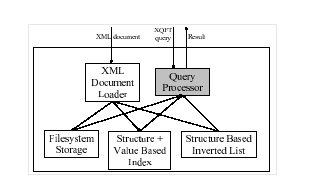
\includegraphics[width=0.5\textwidth]{img/quark_architecture.png}
  \caption{Quark architecture}
\end{figure}
Quark is an experimental full-text search engine capable of indexing and querying XML documents, and it uses the TexQuery query language (see below). Quark was developed as a research project at Cornell University by Jayavel Shanmugasundaram and his associates.
\begin{figure}[!h]
  \centering
    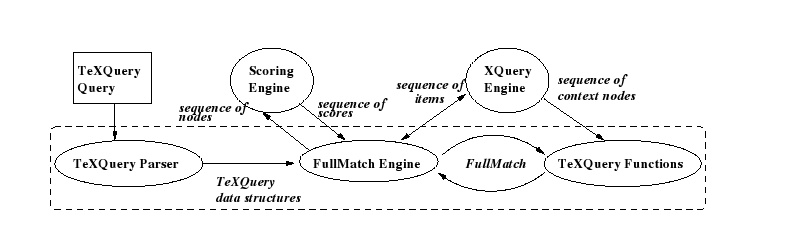
\includegraphics[width=1\textwidth]{img/texquery_architecture.png}
  \caption{TexQuery architecture}
\end{figure}
TexQuery is a query language extending upon Xquery with added full-text search capabilities. These extensions do not necessarily conform to the W3C recommendation, however TexQuery is an early precursor to the current W3C recommendation \cite{TEXQ00}, in whose development Shanmugasundaram actively participates.

\subsubsection{Galatex}
\begin{figure}[!h]
  \centering
    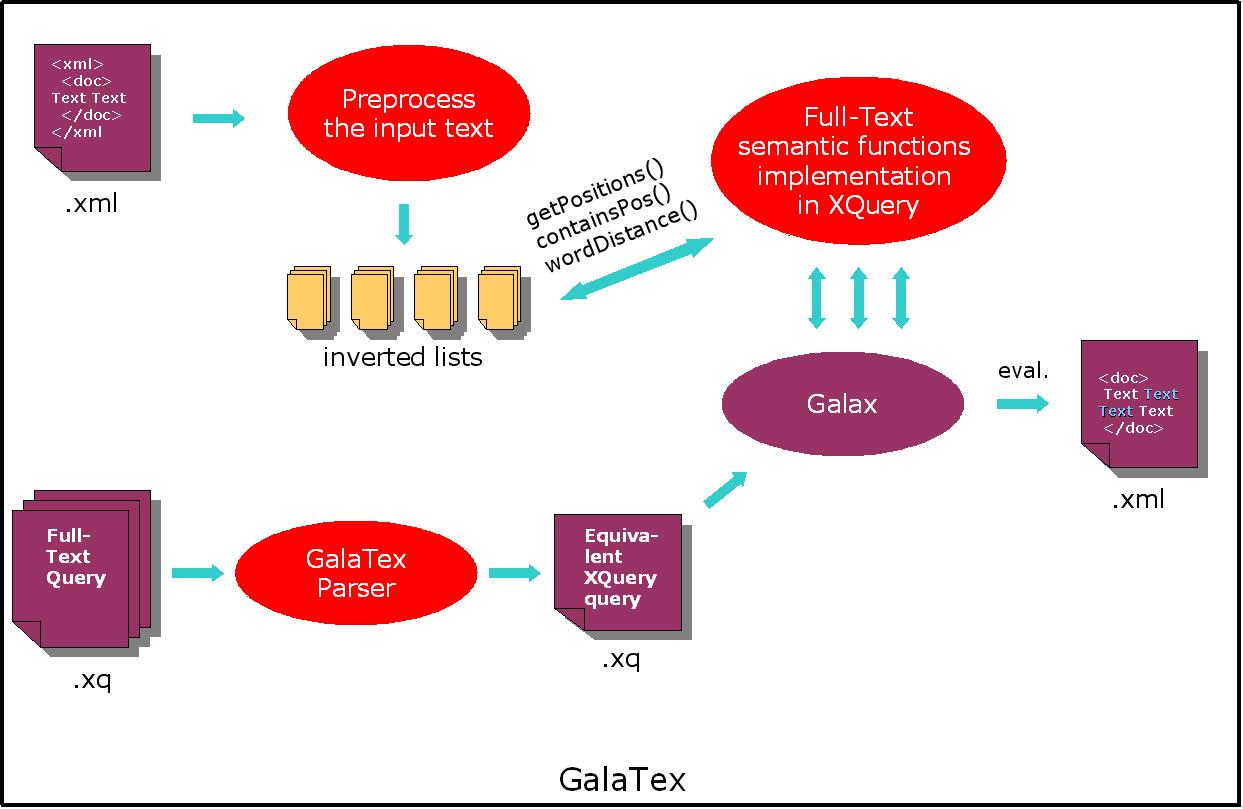
\includegraphics[width=1\textwidth]{img/galatex_architecture.png}
  \caption{Galatex architecture}
\end{figure}
GalaTex is a complete implementation of the Xquery 1.0 and Xpath 2.0
specifications with full-text extensions. GalaTex is an extension of Galax,
which is a generic Xquery engine. The XQFT query is parsed and converted to an
equivalent Xquery query which is passed to the Galax query engine. The GalaTex
source code is licensed under a non-commercial license developed to AT\&{}T 
\footnote{http://www.galaxquery.com/galatex/LICENSE} and is available at the
GalaTex website \cite{galatex}.

\subsubsection{Pathfinder}
\begin{figure}[!h]
  \centering
    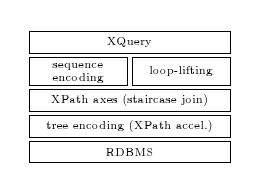
\includegraphics[width=0.5\textwidth]{img/pathfinder_architecture.png}
  \caption{Pathfinder architecture / development stack}
\end{figure}
The Pathfinder project is an XQuery parser running on top of relational database systems, namely MonetDB. The goal of the Pathfinder project is to investigate how relational database technology can be utilized to create a scalable and efficient XQuery implementation. However, the Pathfinder project has, at the current time of writing, no support for full text extensions. A future version of Pathfinder is planned to be capable of emitting SQL code generated from the XQuery parse tree. This illustrates the Pathfinder systems capabilities of interoperating with relational database systems.

Pathfinder is written in C, and the XQuery parser is a generated using standard Flex and Bison compiler generator tools.

\subsubsection{SaXon}
SaXon is an open source XSLT and XQuery processor. It is being actively developed by Michael Kay, and is licensed under the Mozilla Public License (MPL). SaXon conforms to the XSLT 2.0, XQuery 1.0 and XPath 2.0 recommendations by the W3C as of 23rd of january, 2007.

\subsubsection{Natix}
\begin{figure}[!h]
  \centering
    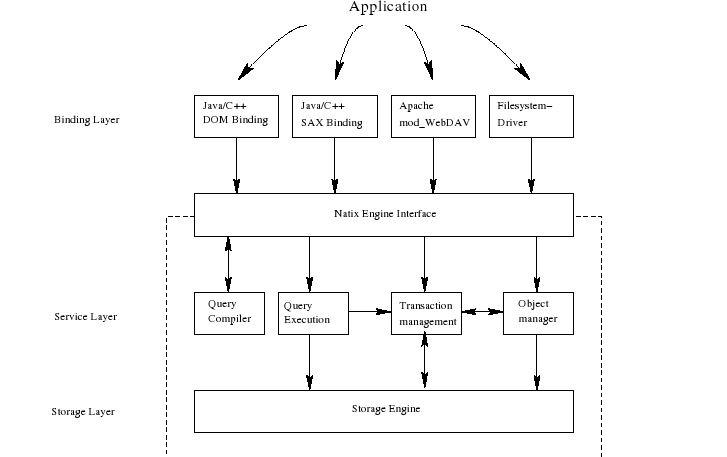
\includegraphics[width=1\textwidth]{img/natix_architecture.png}
  \caption{Natix architecture}
\end{figure}
Natix is an XML database system for persistent storage of XML, and provides access through DOM and SAX interfaces, as well as the option of performing XPath queries.

\section{Summary}
In this chapter, we have presented the basic facets of XQuery and XPath,
especially language features such as FLWOR constructs, path expressions, 
full-text extensions, and precedence. This creates a context for the subsequent
chapters where we will set out to create an XQuery parser with full-text
extensions. 

Further we have investigated existing implementations, both with and without
full-text extensions. These implementations will provide valuable points of
reference for our implementation in the following chapters.

In the next chapter, we will outline the architectural decisions made in this
project.